\documentclass[thesis.tex]{subfiles}

\begin{document}
\chapter{Results}
\section{Proof of concept}
This section can be seen as an introduction to the usage of the tool in Appendix \ref{ref:tool} as much as it is a display of results. Even though this thesis is mainly concerned with the conceptual algorithm and not the implemented tool, every test case starts with the commands which is run to produce the graphical output. This is mainly done to clearly show the input data going in to the experiments, but also as introductionary examples to users of the tool. 
\par\noindent
We start out by building a graph from a single sequence:\\
\begin{figure}[H]
  \begin{mdframed}
    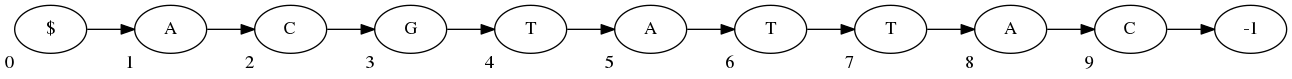
\includegraphics[width=\textwidth]{outputs/equal-merge.png}
  \end{mdframed}
  \caption{A reference graph made from the sequence ``ACGTATTAC''}
  \label{fig:output_ref}
\end{figure}
\subsection{Equal sequences}
\begin{figure}[H]
  \begin{subfigure}[t]{\textwidth}
    \begin{mdframed}
      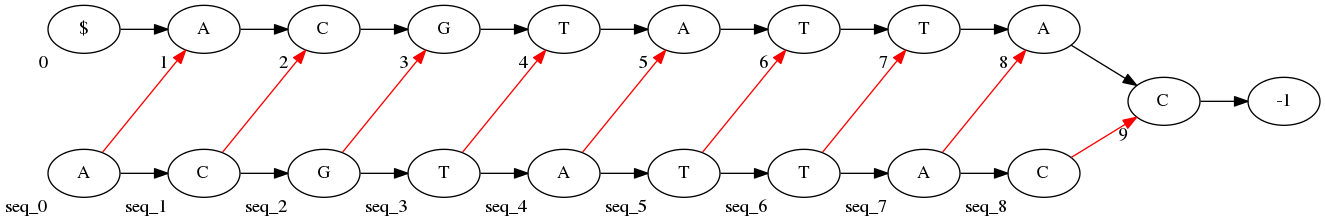
\includegraphics[width=\textwidth]{outputs/equal-alignment.png}
    \end{mdframed}
    \subcaption{}
  \end{subfigure}
  \begin{subfigure}[t]{\textwidth}
    \begin{mdframed}
      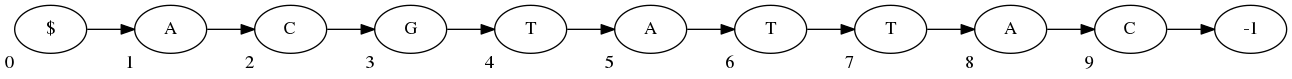
\includegraphics[width=\textwidth]{outputs/equal-merge.png}
    \end{mdframed}
    \subcaption{}
  \end{subfigure}
  \caption{The result of aligning (a) and merging (b) the sequence ``ACGTATTAC'' against the reference graph seen in Fig. \ref{fig:output_ref}}
  \label{fig:output_equal}
\end{figure}
\subsection{SNPs}
\begin{figure}[H]
  \begin{subfigure}[t]{\textwidth}
    \begin{mdframed}
      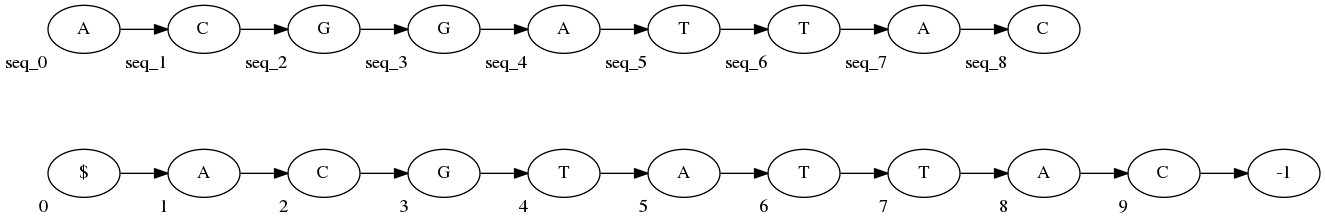
\includegraphics[width=\textwidth]{outputs/snp-no-margin-alignment.png}
    \end{mdframed}
    \subcaption{}
  \end{subfigure}
  \begin{subfigure}[t]{\textwidth}
    \begin{mdframed}
      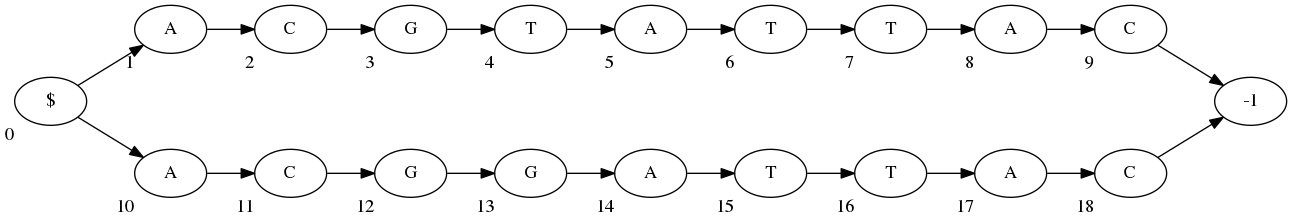
\includegraphics[width=\textwidth]{outputs/snp-no-margin-merge.png}
    \end{mdframed}
    \subcaption{}
  \end{subfigure}
 \caption{The result of aligning (a) and merging (b) the sequence ``ACGGATTAC'' against the reference graph seen in Fig. \ref{fig:output_ref} with $\lambda=0$}
\end{figure}
\begin{figure}[H]
  \begin{subfigure}[t]{\textwidth}
    \begin{mdframed}
      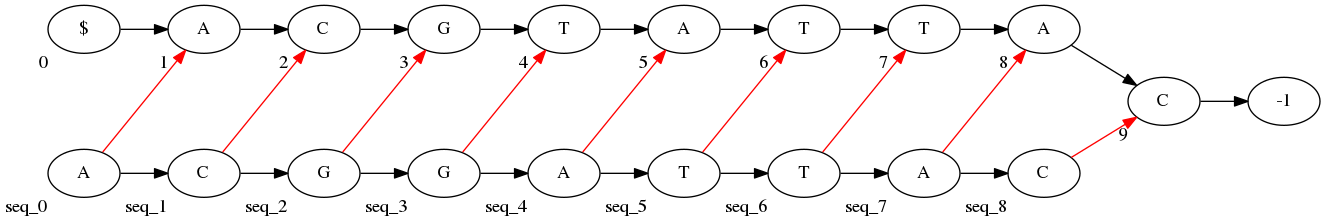
\includegraphics[width=\textwidth]{outputs/snp-alignment.png}
    \end{mdframed}
    \subcaption{}
  \end{subfigure}
  \begin{subfigure}[t]{\textwidth}
    \begin{mdframed}
      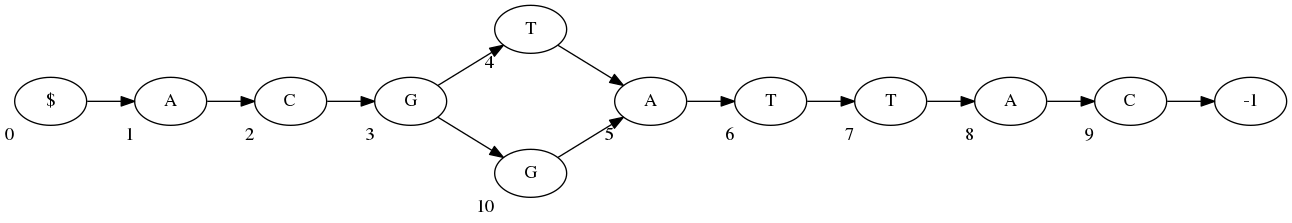
\includegraphics[width=\textwidth]{outputs/snp-merge.png}
    \end{mdframed}
    \subcaption{}
  \end{subfigure}
  \begin{subfigure}[t]{\textwidth}
    \begin{mdframed}
      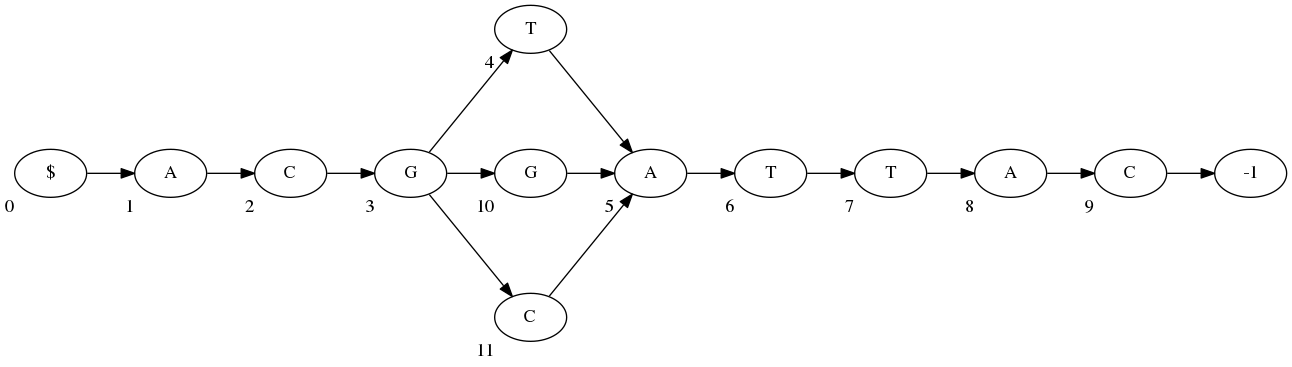
\includegraphics[width=\textwidth]{outputs/snp-merge-two.png}
    \end{mdframed}
    \subcaption{}
  \end{subfigure}
  \caption{The result of aligning (a) and merging (b) the sequence ``ACGGATTAC'' against the reference graph seen in Fig. \ref{fig:output_ref} and then merging the sequence ``ACGCATTAC'' (c) with $\lambda=1$}
  \label{fig:output_snp}
\end{figure}
\subsection{Indels}
\begin{figure}[H]
  \begin{subfigure}[t]{\textwidth}
    \begin{mdframed}
      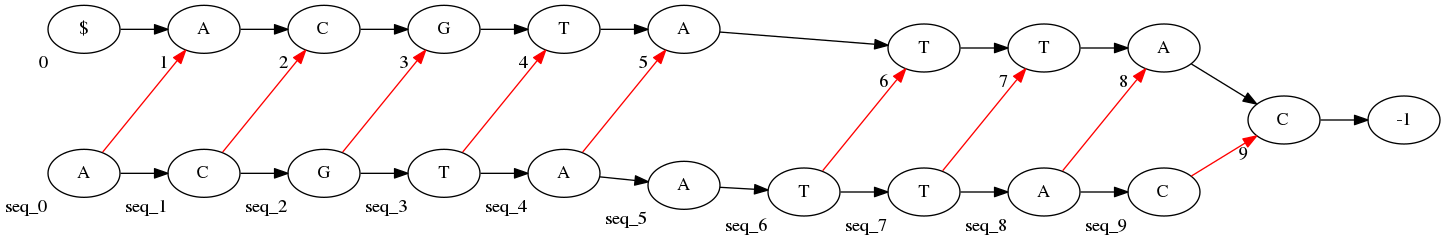
\includegraphics[width=\textwidth]{outputs/insertion-alignment.png}
    \end{mdframed}
    \subcaption{}
  \end{subfigure}
  \begin{subfigure}[t]{\textwidth}
    \begin{mdframed}
      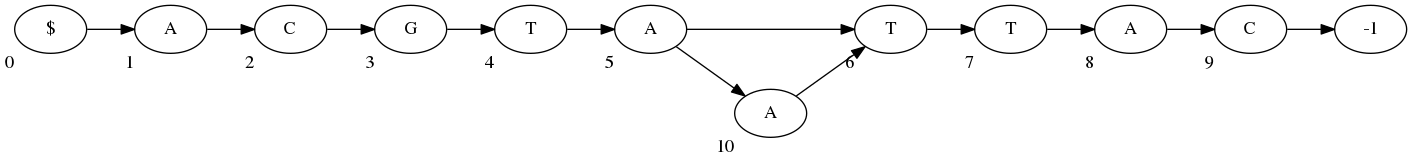
\includegraphics[width=\textwidth]{outputs/insertion-merge.png}
    \end{mdframed}
    \subcaption{}
  \end{subfigure}
  \caption{The result of aligning (a) and merging (b) the sequence ``ACGTAATTAC'' against the reference graph seen in Fig. \ref{fig:output_ref}}
  \label{fig:output_insertion}
\end{figure}
\begin{figure}[H]
  \begin{subfigure}[t]{\textwidth}
    \begin{mdframed}
      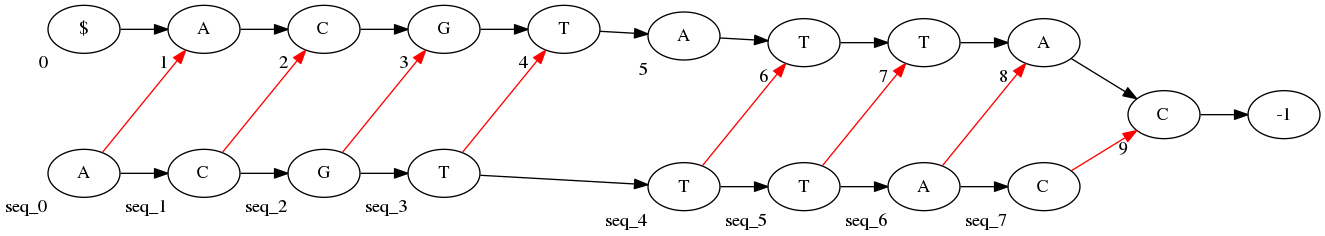
\includegraphics[width=\textwidth]{outputs/deletion-alignment.png}
    \end{mdframed}
    \subcaption{}
  \end{subfigure}
  \begin{subfigure}[t]{\textwidth}
    \begin{mdframed}
      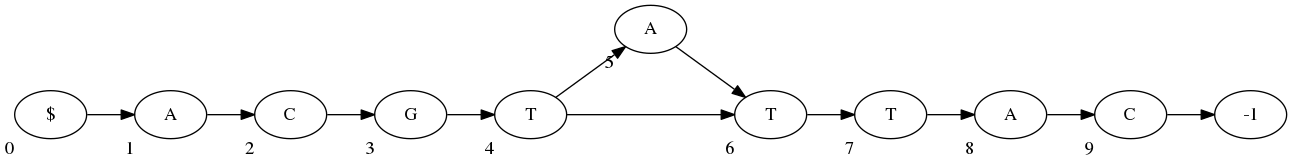
\includegraphics[width=\textwidth]{outputs/deletion-merge.png}
    \end{mdframed}
    \subcaption{}
  \end{subfigure}
  \caption{The result of aligning (a) and merging (b) the sequence ``ACGTTTAC'' against the reference graph seen in Fig. \ref{fig:output_ref}}
  \label{fig:output_deletion}
\end{figure}
\subsection{Structural variations}
\section{Efficiency}
\subsection{Building the index}
\subsection{Alignment}
\subsubsection{Runtime as a function of |G|}
\subsubsection{Runtime as a function of |s|}
\subsubsection{Runtime as a function of $\lambda$}
\end{document}